\documentclass{article}

% Russian language
\usepackage[utf8]{inputenc}
\usepackage[russian]{babel}

\usepackage{biblatex}       % for roman digits

\usepackage{amsmath, amssymb}
\usepackage[left=20mm, right=20mm, top=2cm]{geometry}
\usepackage{array}

\usepackage{graphicx}
\usepackage{ragged2e}
\usepackage{wrapfig}
\justifying

\graphicspath{{images/}}

\title{
    \textbf{Лабораторная работа 3.4.5}
}
\author{Герасименко Д.В.}
\date{2 курс ФРКТ, группа Б01-104}

\begin{document}

\maketitle

\begin{center}
    \raggedleft
        \underline{\underline{\LARGE {Аннотация}}}
\end{center}

\begin{center}
\raggedright
    \large{\textbf{Тема:}}
    \\
    \large {Петля гистерезиса (динамический метод)}
    
    \large{\textbf{Цель работы:}}
    \\
    \large {Изучение петель гистерезиса различных ферромагнитных материалов в переменных полях}
    
    \large{\textbf{Оборудование:}}
    \\
    \large{автотрансформатор, понижающий трансформатор, интегрирующая цепочка, амперметр, вольтметр, электронный
    осциллограф, делитель напряжения, тороидальные образцы с двумя обмотками.}
\end{center}

\begin{center}
    \raggedleft
        \underline{\underline{\LARGE {Теория}}}
\end{center}

Основные характеристики ферромагнетиков — их коэрцитивное поле $H_c$, магнитная проницаемость $\mu$, рассеиваемая в виде тепла при перемагничивании мощность — зависят от частоты перемагничивающего поля. В данной работе кривые гистерезиса ферромагнитных материалов изучаются в поле частоты $\nu_0 =$ 50 Гц с помощью электронного осциллографа.

\begin{center}
    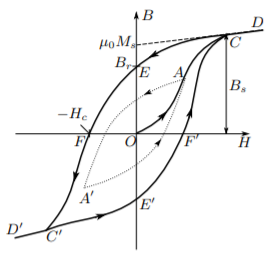
\includegraphics[width = 0.4\textwidth]{petlya.png} \\
	\textbf{Рис. 1.} Петля гистерезиса ферромагнетика
\end{center}

Магнитная индукция $ B $ и напряжённость поля $ H $ в ферромагнитном материале неоднозначно связаны между собой: индукция зависит не только от напряжённости, но и от предыстории образца. Связь между $ B $ и $ H $ типичного ферромагнетика иллюстрирует рис. 1.

Если к ферромагнитному образцу прикладывать переменное внешнее магнитное поле, то его состояние на плоскости $ B-H $ будет изменяться по замкнутой кривой — петле гистерезиса. Размер петли определяется максимальным значением напряжённости $ H $ в цикле (например, петля $ AA' $, обозначенная пунктиром на рис. 1). Если амплитуда напряжённости достаточно велика, то образец будет периодически достигать насыщения, что на рисунке соответствует кривой $ CEFC'E'F'C $ (предельная петля гистерезиса). Пересечение предельной петли с вертикальной осью соответствует остаточной индукции $B_r$, пересечение с горизонтальной осью — коэрцитивному полю $H_c$. Крайние точки петель, соответствующие амплитудным значениям $ H $ (например, точка $ A $ на рис. 1), лежат на начальной кривой намагничивания ($ OAC $).

\textbf{Измерение магнитной индукции.} Магнитную индукцию $ B $ удобно определять с помощью ЭДС, возникающей при изменении магнитного потока $ \Phi $ в катушке, намотанной на образец. Пусть катушка c $ N $ витками плотно охватывает образец сечением $ S $, и индукция $ B $ в образце однородна. Тогда

\begin{equation}
    |B|=\frac{1}{SN}\int\mathcal{E} dt.
\end{equation}

\begin{center}
    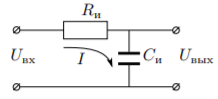
\includegraphics[width=0.4\textwidth]{int.png} \\
    \textbf{Рис. 2.} Интегрирующая ячейка
\end{center}

Для интегрирования в работе используется интегрирующая $ RC $-цепочка (рис. 2). «Входное» напряжение от источника $U_{\text{вх}}(t)$ подаётся на последовательно соединённые резистор $R_\text{и}$ и конденсатор $C_\text{и}$. <<Выходное>> напряжение $U_{\text{вых}}(t)$ снимается с конденсатора. Предположим, что 1) сопротивление источника мало по сравнению с $R_\text{и}$, 2) выходное сопротивление (сопротивление на входе осциллографа), напротив, велико: $R_{\text{вых}}$ $ \gg $ $R_\text{и}$ и, наконец, 3) сопротивление $R_\text{и}$ достаточно велико, так что почти всё падение напряжения приходится на него, а $U_{\text{вых}}$ $\ll$ $U_{\text{вх}}$. В таком случае ток цепи равен I = ($U_{\text{вх}}$ - $U_{\text{вых}}$)/$R_\text{и}$ $\approx$ $U_{\text{вх}}$/$R_\text{и}$, и входное и выходное сопротивление связаны соотношением

\begin{equation}
    U_{\text{вых}} = \frac{q}{C_\text{и}} = \frac{1}{C_\text{и}}\int\limits_0^t Idt \approx \frac{1}{\tau_\text{и}} \int\limits_0^t U_{\text{вх}}dt,
    \label{eq:U_ext}
\end{equation}

где $\tau_\text{и}=R_\text{и}C_\text{и}$ - постоянная времени $ RC $ - цепочки. Для индукции поля из (1) получаем 

\begin{equation}
    |B|=\frac{1}{SN}\int U_{\text{вх}} dt=\frac{\tau_\text{и}}{SN}U_{\text{вых}}.
    \label{eq:|B|new}
\end{equation}

\fbox{
\parbox[t][1.01\height]{17cm} 
{%
\textbf{Замечание.} Уточним критерий применимости соотношения ($\ref{eq:U_ext}$). Пусть на вход интегрирующей ячейки подан синусоидальный сигнал с частотой $\omega_0$. Тогда, пользуясь методом комплексных амплитуд, нетрудно найти отношение амплитуд входного и выходного напряжений:

\begin{equation}
    \frac{U_{\text{вых}}}{U_{\text{вх}}}=\frac{1/\omega_0C}{\sqrt{R^2+1/(\omega_0C)^2}}.
\end{equation}

Тогда неравенство $U_{\text{вых}} \ll U_{\text{вх}}$ реализуется, если 
\begin{equation}
    \tau \equiv RC\gg \frac{1}{\omega_0}
\end{equation}
(импеданс конденсатора мал по сравнению сопротивлением резистора). В таком случае для синусоидального сигнала имеем

\begin{equation}
    \frac{U_{\text{вых}}}{U_{\text{вх}}}\approx\frac{1}{\omega_0\tau}.
\end{equation}

В общем случае, если $\omega_0$ — частота самой низкой гармоники в спектре произвольного входного сигнала, то при $\omega_0\tau \gg 1$ неравенство $U_{\text{вых}} \ll U_{\text{вх}}$ выполняется на любой частоте $\omega > \omega_0$.}}

\begin{center}
    \raggedleft
        \underline{\underline{\LARGE {Экспериментальная установка}}}
\end{center}

Схема установки изображена на рис. 3. Напряжение сети (220 В,
50 Гц) с помощью трансформаторного блока Т, состоящего из регулировочного автотрансформатора и разделительного понижающего трансформатора, подаётся на намагничивающую обмотку $N_0$ исследуемого образца.

\begin{center}
	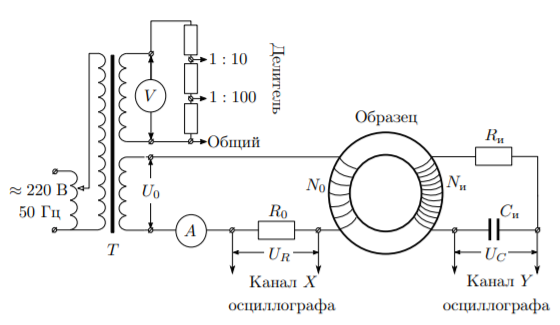
\includegraphics[width=0.7\textwidth]{scheme.png} \\
	\textbf{Рис. 3} Схема установки для исследования намагничивания образцов.
\end{center}

В цепь намагничивающей катушки, на которую подаётся некоторое
напряжение $U_0$, последовательно включено сопротивление $R_0$. Напряжение на $R_0$, равное $U_R$= $R_0I_0$, где $I_0$ — ток в намагничивающей обмотке $N_0$, подаётся на канал $ X $ осциллографа. Связь напряжённости $ H $ в образце и тока $I_0$ рассчитывается по теореме о циркуляции.  Действующее значение переменного тока в обмотке $N_0$ измеряется амперметром A. Для измерения магнитной индукции $ B $ с измерительной обмотки $N_\text{и}$ на вход $ RC $-цепочки подаётся напряжение $U_\text{и}$ ($U_{\text{вх}}$), пропорциональное производной $ dB/dt $. С интегрирующей ёмкости $C_\text{и}$ снимается напряжение $U_C$ ($U_{\text{вых}}$), пропорциональное величине $ B $, и подаётся на вход $ Y $ осциллографа. Значение индукции поля $ B $ рассчитывается по формуле (3). Замкнутая кривая, возникающая на экране, воспроизводит в некотором масштабе (различном для осей $ X $ и $ Y $) петлю гистерезиса. Чтобы придать этой кривой количественный смысл, необходимо установить масштабы изображения, т. е. провести калибровку каналов $ X $ и $ Y $ осциллографа.

\begin{center}
    \raggedleft
        \underline{\underline{\LARGE {Выполнение}}}
\end{center}

\begin{center}
    \underline{\large {\RN{1}. Измерение петли резонанса}}
\end{center}

1) Соберем схему согласно рис. 3. Подберем ток питания в намагничивающей обмотке с помощью автотрансформатора и коэффициенты усиления ЭО таким образом, чтобы предельная петля гистерезиса занимала большую часть экрана. Приведем характерные значения катушек разных материалов в таблице 1.

\begin{center}
    \begin{tabular}{|c|c|c|c|c|}
		\hline
		Материал     & $N_0$ & $N_\text{и}$ & $S^2$, см$^2$ & $2\pi R$, см \\ \hline
		Феррит       & 40    & 400          & 3.0           & 25.0         \\ \hline
		Пермаллой    & 35    & 220          & 3.8           & 24.0         \\ \hline
		Крем. железо & 40    & 400          & 1.2           & 10.0         \\ \hline
	\end{tabular}
	
	\textbf{Таблица 1.} Характеристики катушек
\end{center}

2) Для каждого образца получим передельные петли гистерезиса, по коэффициентам усиления ЭО $K_x$ и $K_y$ рассчитаем масштабы, определим двойные амплитуды коэрцетивной силы $ [2x(c)] $ и индукции насыщения $ [2y(s)] $. Масштабы по осям $ X $ и $ Y $ рассчитаем по формулам  $H=IN_0/(2\pi R),\ где\ I=K_x/R_0;\ B=R_\text{и}C_\text{и}U_{\text{вых}}/(SN_\text{и}),$ где $U_{\text{вых}}=K_y$. Результаты измерений и вычислений занесём в таблицу 2.

\begin{center}
    \begin{tabular}{|c|c|c|c|c|c|c|c|c|c|}
        \hline
        Материал & \([2X_{s}]\), дел & \([2Y_{s}]\), дел & \([2X_{c}]\), дел & \([2Y_{c}]\), дел & \(K_{x}, \frac{\text{мВ}}{\text{дел}}\) & \(K_{y} \frac{\text{мВ}}{\text{дел}}\) & \(I_{\text{эфф}}\), мА & \(H, \frac{\text{A}}{\text{м дел}}\) & \(B, \frac{\text{Тл}}{\text{дел}}\) \\
        \hline
        Феррит & 6.4 & 4.0 & 1.2 & 1.7 & 20 & 20 & 127 & 10.6 & 0.07 \\
        \hline
        Пермаллой & 2.9 & 4.3 & 2.1 & 4,0 & 50 & 100 & 170 & 24.3 & 0.48 \\
        \hline
        Железо & 4.8 & 5.8 & 1.6 & 2.1 & 50 & 50 & 244 & 66.7 & 0.42 \\
        \hline
    \end{tabular}
    
    \textbf{Таблица 2} Для измерительных шкалы для материалов
\end{center}

3) Зная масштабы по осям, можно определить значения коэрцетивной силы $ H_c $ и индукции насыщения $ B_s $. Результаты заносим в таблицу 3. Рассчитаем погрешности соответствующих величин из формул для них:

\begin{equation}
    H_{c} = \frac{[2X_{c}]}{2} \cdot H = [X_{c}] \cdot \frac{N_{0}}{2\pi R} \frac{K_{x}}{R_{0}} \Rightarrow \sigma_{H_{c}} = \sigma_{[X_{c}]} \hspace{1cm}
    B_{s} = \frac{[2Y_{s}]}{2} \cdot B = [Y_{s}] \cdot \frac{R_{u}C_{u}}{S N_{u}} K_{y} \Rightarrow \sigma_{B_{s}} = \sigma_{[Y_{s}]}
\end{equation}

\begin{center}
    \begin{tabular}{|c|c|c|c|c|}
		\hline
		Материал     & $H_c$, \(\frac{\text{А}}{\text{м}}\) & $\sigma_{H_c}$,  \(\frac{\text{А}}{\text{м}}\) & $B_s$,  мТл & $\sigma_{B_s}$, мТл \\ \hline
		Феррит       & 6.4       & 1.1                 & 60      & 7              \\ \hline
		Пермаллой    & 25.5      & 2.4                & 1032      & 48               \\ \hline
		Крем. железо & 53.4      & 6.7                & 1218      & 42               \\ \hline
	\end{tabular}
	
	\textbf{Таблица 3.} Результаты вычислений
\end{center}

4) Для каждого из образцов построим начальные кривые гистерезиса, сняв 8 измерний.

\begin{center}
    \begin{tabular}{|c|c|c|c|c|c|c|c|c|}
        \hline
        I, мА & 118 & 109 & 96 & 86 & 77 & 63 & 49 & 38 \\
        \hline
        \([2X_{s}]\), дел & 6.1 & 5.9 & 4.9 & 4.3 & 3.8 & 3.0 & 2.4 & 1.8 \\
        \hline
        \([2Y_{s}]\), дел & 4.0 & 3.9 & 3.7 & 3.4 & 3.2 & 2.8 & 2.2 & 1.6 \\
        \hline
        \(B\), Тл & 0.14 & 0.14 & 0.13 & 0.12 & 0.11 & 0.10 & 0.08 & 0.06 \\
        \hline
        \(H, \frac{\text{А}}{\text{м}}\) & 32.33 & 31.27 & 25.97 & 22.79 & 20.14 & 15.90 & 12.72 & 9.54 \\
        \hline
    \end{tabular}
    
    \textbf{Таблица 4.1.} Начальная кривая для феррита
\end{center}
    
\begin{center}
    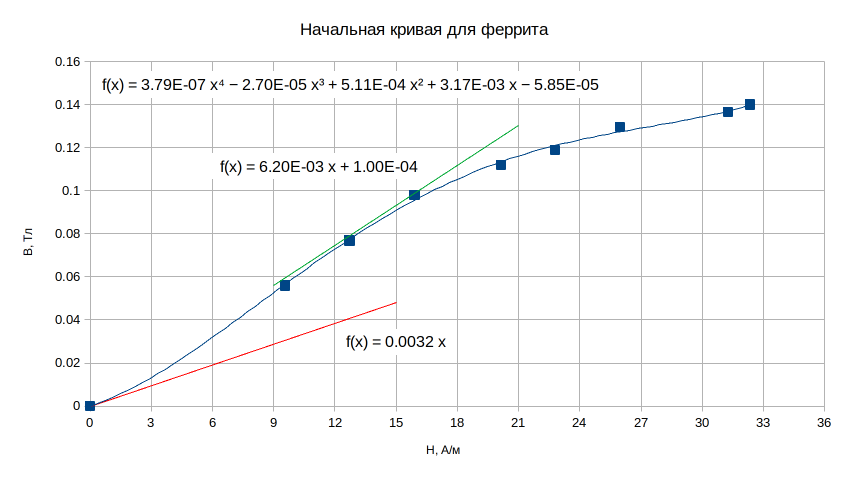
\includegraphics[width = 0.8\textwidth]{curve_init_f.png}
    
    \textbf{Рис 1.1.} Начальная кривая феррита
\end{center}

Соответствующие значения 

\begin{equation*}
    \mu_{\text{диф}}(0) = (3.2 \pm 0.6) \cdot 10^{-3} \frac{\text{Тл м}}{\text{А}} \hspace{1cm} \mu_{max} = (6.2 \pm 1.2) \cdot 10^{-3} \frac{\text{Тл м}}{\text{А}}
\end{equation*}

\begin{center}
    \begin{tabular}{|c|c|c|c|c|c|c|c|c|}
        \hline
        I, мА & 152 & 140 & 130 & 120 & 110 & 100 & 90 & 80 \\
        \hline
        \([2X_{s}]\), дел & 2.3 & 2.1 & 1.9 & 1.7 & 1.5 & 1.2 & 1.0 & 0.6 \\
        \hline
        \([2Y_{s}]\), дел & 4.0 & 3.8 & 3.4	& 3.0 & 2.5	& 1.6 & 1.1 & 0.4 \\
        \hline
        \(B\), Тл & 0.84 & 0.80 & 0.71 & 0.63 & 0.53  & 0.34 & 0.23 & 0.084 \\
        \hline
        \(H, \frac{\text{А}}{\text{м}}\) & 76.71 & 70.04 & 63.37 & 56.70 & 50.03 & 40.02 & 33.35 & 20.01 \\
        \hline
    \end{tabular}
    
    \textbf{Таблица 4.2.} Начальная кривая для пермаллоя
\end{center}

\begin{center}
    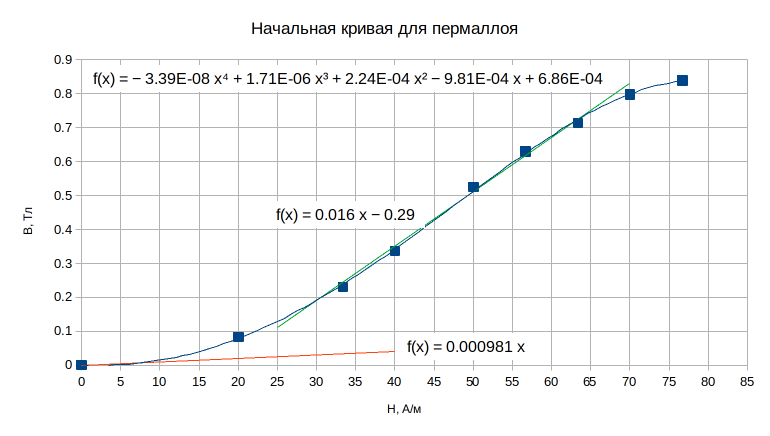
\includegraphics[width=0.8\textwidth]{curve_init_p.png}
    
    \textbf{Рис 1.2.} Начальная кривая для пермаллоя 
\end{center}

Соответствующие значения 

\begin{equation*}
    \mu_{\text{диф}}(0) \approx (10 \pm 2) \cdot 10^{-4} \frac{\text{Тл м}}{\text{А}} \hspace{1cm} \mu_{max} = (16 \pm 3) \cdot 10^{-3} \frac{\text{Тл м}}{\text{А}}
\end{equation*}

\newpage

\begin{center}
    \begin{tabular}{|c|c|c|c|c|c|c|c|c|}
        \hline
        I, мА & 221 & 191 & 181 & 171 & 162 & 152 & 133 & 120 \\
        \hline
        \([2X_{s}]\), дел & 4.4 & 3.7 & 3.5 & 3.3 & 3.2 & 2.9 & 2.5 & 2.3 \\
        \hline
        \([2Y_{s}]\), дел & 5.5 & 5.1 & 4.8 & 4.6 & 4.5 & 4.2 & 3.8 & 3.4 \\
        \hline
        \(B\), Тл & 1.32 & 1.22	& 1.15 & 1.11 & 1.08 & 1.01 & 0.91 & 0.82 \\
        \hline
        \(H, \frac{\text{А}}{\text{м}}\) & 53.46 & 44.96 & 42.53 & 40.10 & 38.88 & 35.24 & 30.38 & 27.95 \\
        \hline
    \end{tabular}
    
    \textbf{Таблица 4.3.} Начальная кривая для кремниевого железа
\end{center}

\begin{center}
    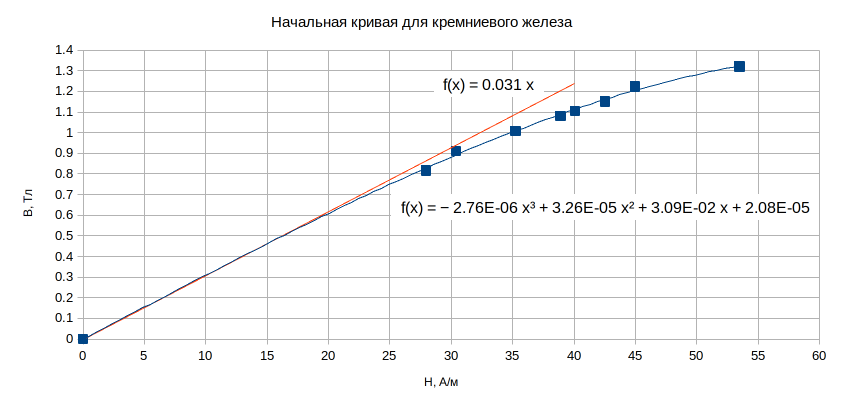
\includegraphics[width=0.8\textwidth]{curve_init_ferrum.png}
    
    \textbf{Рис 1.3.} Начальная кривая для кремниевого железа
\end{center}

Соответствующее значение 

\begin{equation*}
    \mu_{\text{диф}}(0) \approx \mu_{max} = (31 \pm 6) \cdot 10^{-3} \frac{\text{Тл м}}{\text{А}}
\end{equation*}

\begin{center}
    \underline{\large {\RN{2}. Проверка калибровки осциллографа}}
\end{center}

Проверим калибровку ЭО по оси X. Отключим намагничивающую обмотку $N_0$ от цепи, соединив оба провода, идущих к обмотке, на одной ее клемме. С помощью автотрансформатора подберем такой ток через $R_0$, при котором горизонтальная прямая занимает большую часть экрана. При $ K_x=50 \text{ мВ/дел} $ рассчитаем чувствительность $m_x=48.5 \text{ мВ/дел}$.

Аналогичные действия проводим при $ K_x =20 \text{ мВ/дел} $. Получаем $ m_x=19.6 \text{ мВ/дел} $.

Так как $m_x \approx K_x$, ЭО откалиброван по оси X корректно.

Также необходимо проверить калибровку по оси $ Y $. Для этого соединим вход Y ЭО с клеммам делителя "1:100 - земля". Не меняя рабочего коэффициента $K_y = 50\text{ мВ/дел}$, подберем с помощью трансформатора напряжение, при котором вертикальная прямая занимает большую часть экрана. Подключим вольтметр V к тем же клеммам делителя и, используя измеренное $U_{\text{эф}}$, рассчитаем чувствительность $m_y=50.5\text{ мВ/дел}$.

Те же действия повторяем при $K_y =20 \text{ В/дел}$. Получаем $m_y=18.4\text{ В/дел}$.

Так как $m_y \approx K_y$, ЭО откалиброван по оси Y корректно.

\begin{center}
    \underline{\large {\RN{3}. Проверка применимости теоретических выкладок}}
\end{center}



Проверим применимость формулы (2). Для этого рассчитаем $\tau$ -- постоянную времени $ RC $-цепочки. Для определения напряжений на входе и выходе интегрирующей ячейки соединим вход ячейки с обмоткой <<6,3 В>> трансформатора. Подключим Y-вход ЭО ко входу интегрирующей ячейки и отключим X-вход ЭО. Подберем такой ток, чтобы вертикальная прямая занимала большую часть экрана, и определим входное напряжение $U_{\text{вх}}=y\cdot K_y=3\ \text{дел} \cdot 2\ \text{В/дел}=6\ \text{В}$. Не меняя тока, подключим Y-вход ЭО к выходу ячейки и аналогичным образом определим $U_{\text{вых}}=y\cdot K_y=\frac{4.7}{2}\ \text{дел} \cdot 20\ \text{мВ/дел}=47\ \text{мВ}$. Рассчитаем $\tau=\frac{U_{\text{вх}}}{\omega U_{\text{вых}}}=\frac{6}{0.047\cdot2\pi\cdot 50}=0,406\ \text{c}$, где $\omega=2\pi\nu$. По определению $\tau_{RC}=R_\text{и}C_\text{и}=0,4\ \text{с}$. Так как $\tau\approx\tau_{RC}$, то условия применимости нашей теории выполнены.

\newpage

\begin{center}
    \raggedleft
        \underline{\underline{\LARGE {Вывод}}}
\end{center}

В ходе данной работы было исследовано явление гистерезиса магнитной индукции ферромагнитов из разных материлов: феррита, пермаллоя и кремниевого железа. С помощью осциллографа наблюдалась картина в координатах U(U), точки которой по 

\begin{center}
    ФОРМУЛАМ
\end{center}

были пропорциональны значениям магнитной индукции \(B\) и магнитной напряженности  \(H\) в торроидальном сечении магнита. Соответственно были получены следующие результаты:

\begin{center}
    \begin{tabular}{|c|c|c|c|c|}
        \hline
        Материал & \(B_{s}\), млТл & \(H_{c}\), \(\frac{\text{A}}{\text{м}}\) & \(\mu_{\text{нач}}\), \(\frac{\text{Тл м}}{\text{А}}\) & \(\mu_{max}\), \(\frac{\text{Тл м}}{\text{А}}\) \\ 
        \hline
        Феррит & \(60 \pm 7\) & \(6.4 \pm 1.1\) & \(3.2 \pm 0.6\) & \(6.2 \pm 1.2\) \\
        Пермаллой & \(1032 \pm 48\) & \(25.5 \pm 2.4\) & \(10 \pm 2\) & \(16 \pm 3\) \\
        Кремниевое железо & \(1218 \pm 42\) & \(53.4 \pm 6.7\) & \(31 \pm 6\) & \(31 \pm 6\) \\
        \hline
    \end{tabular}
\end{center}

\newpage

\begin{center}
    \raggedleft
        \underline{\underline{\LARGE {Приложение}}}
\end{center}

\begin{center}
    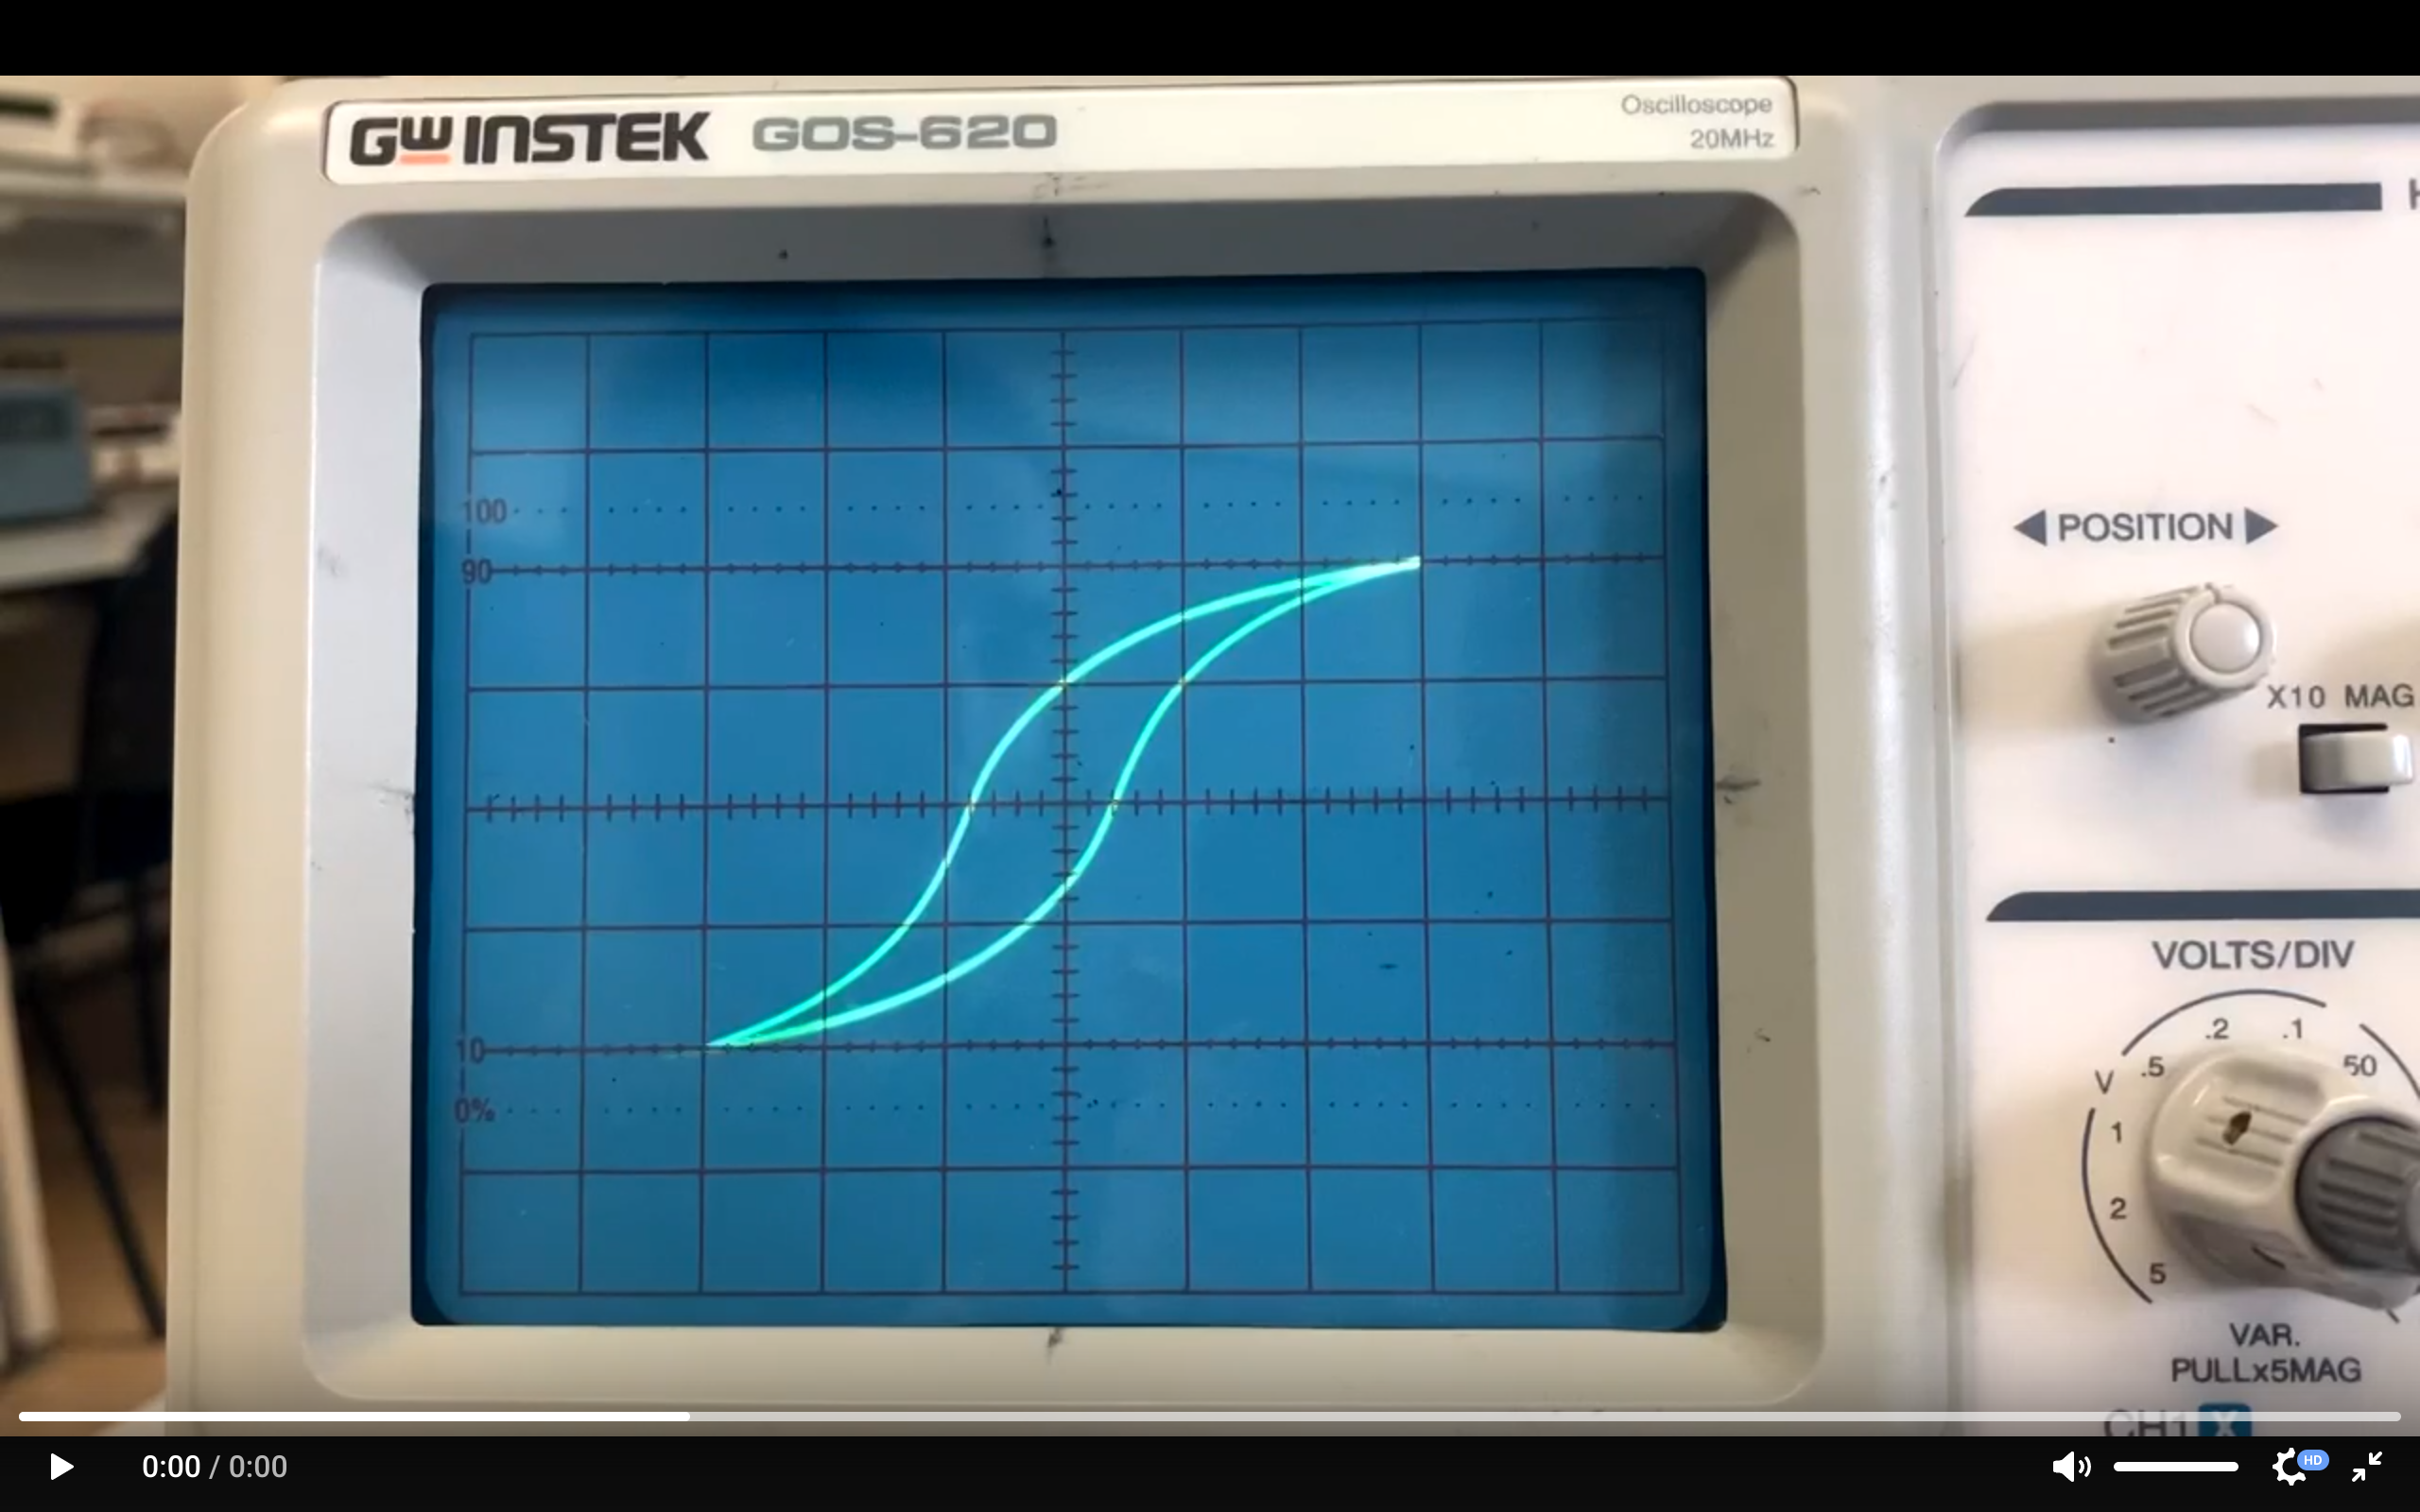
\includegraphics[width=0.55\textwidth]{ferrrit_p.png}
    
    \textbf{Рис 2.1} Петля гистерезиса для феррита
\end{center}

\begin{center}
    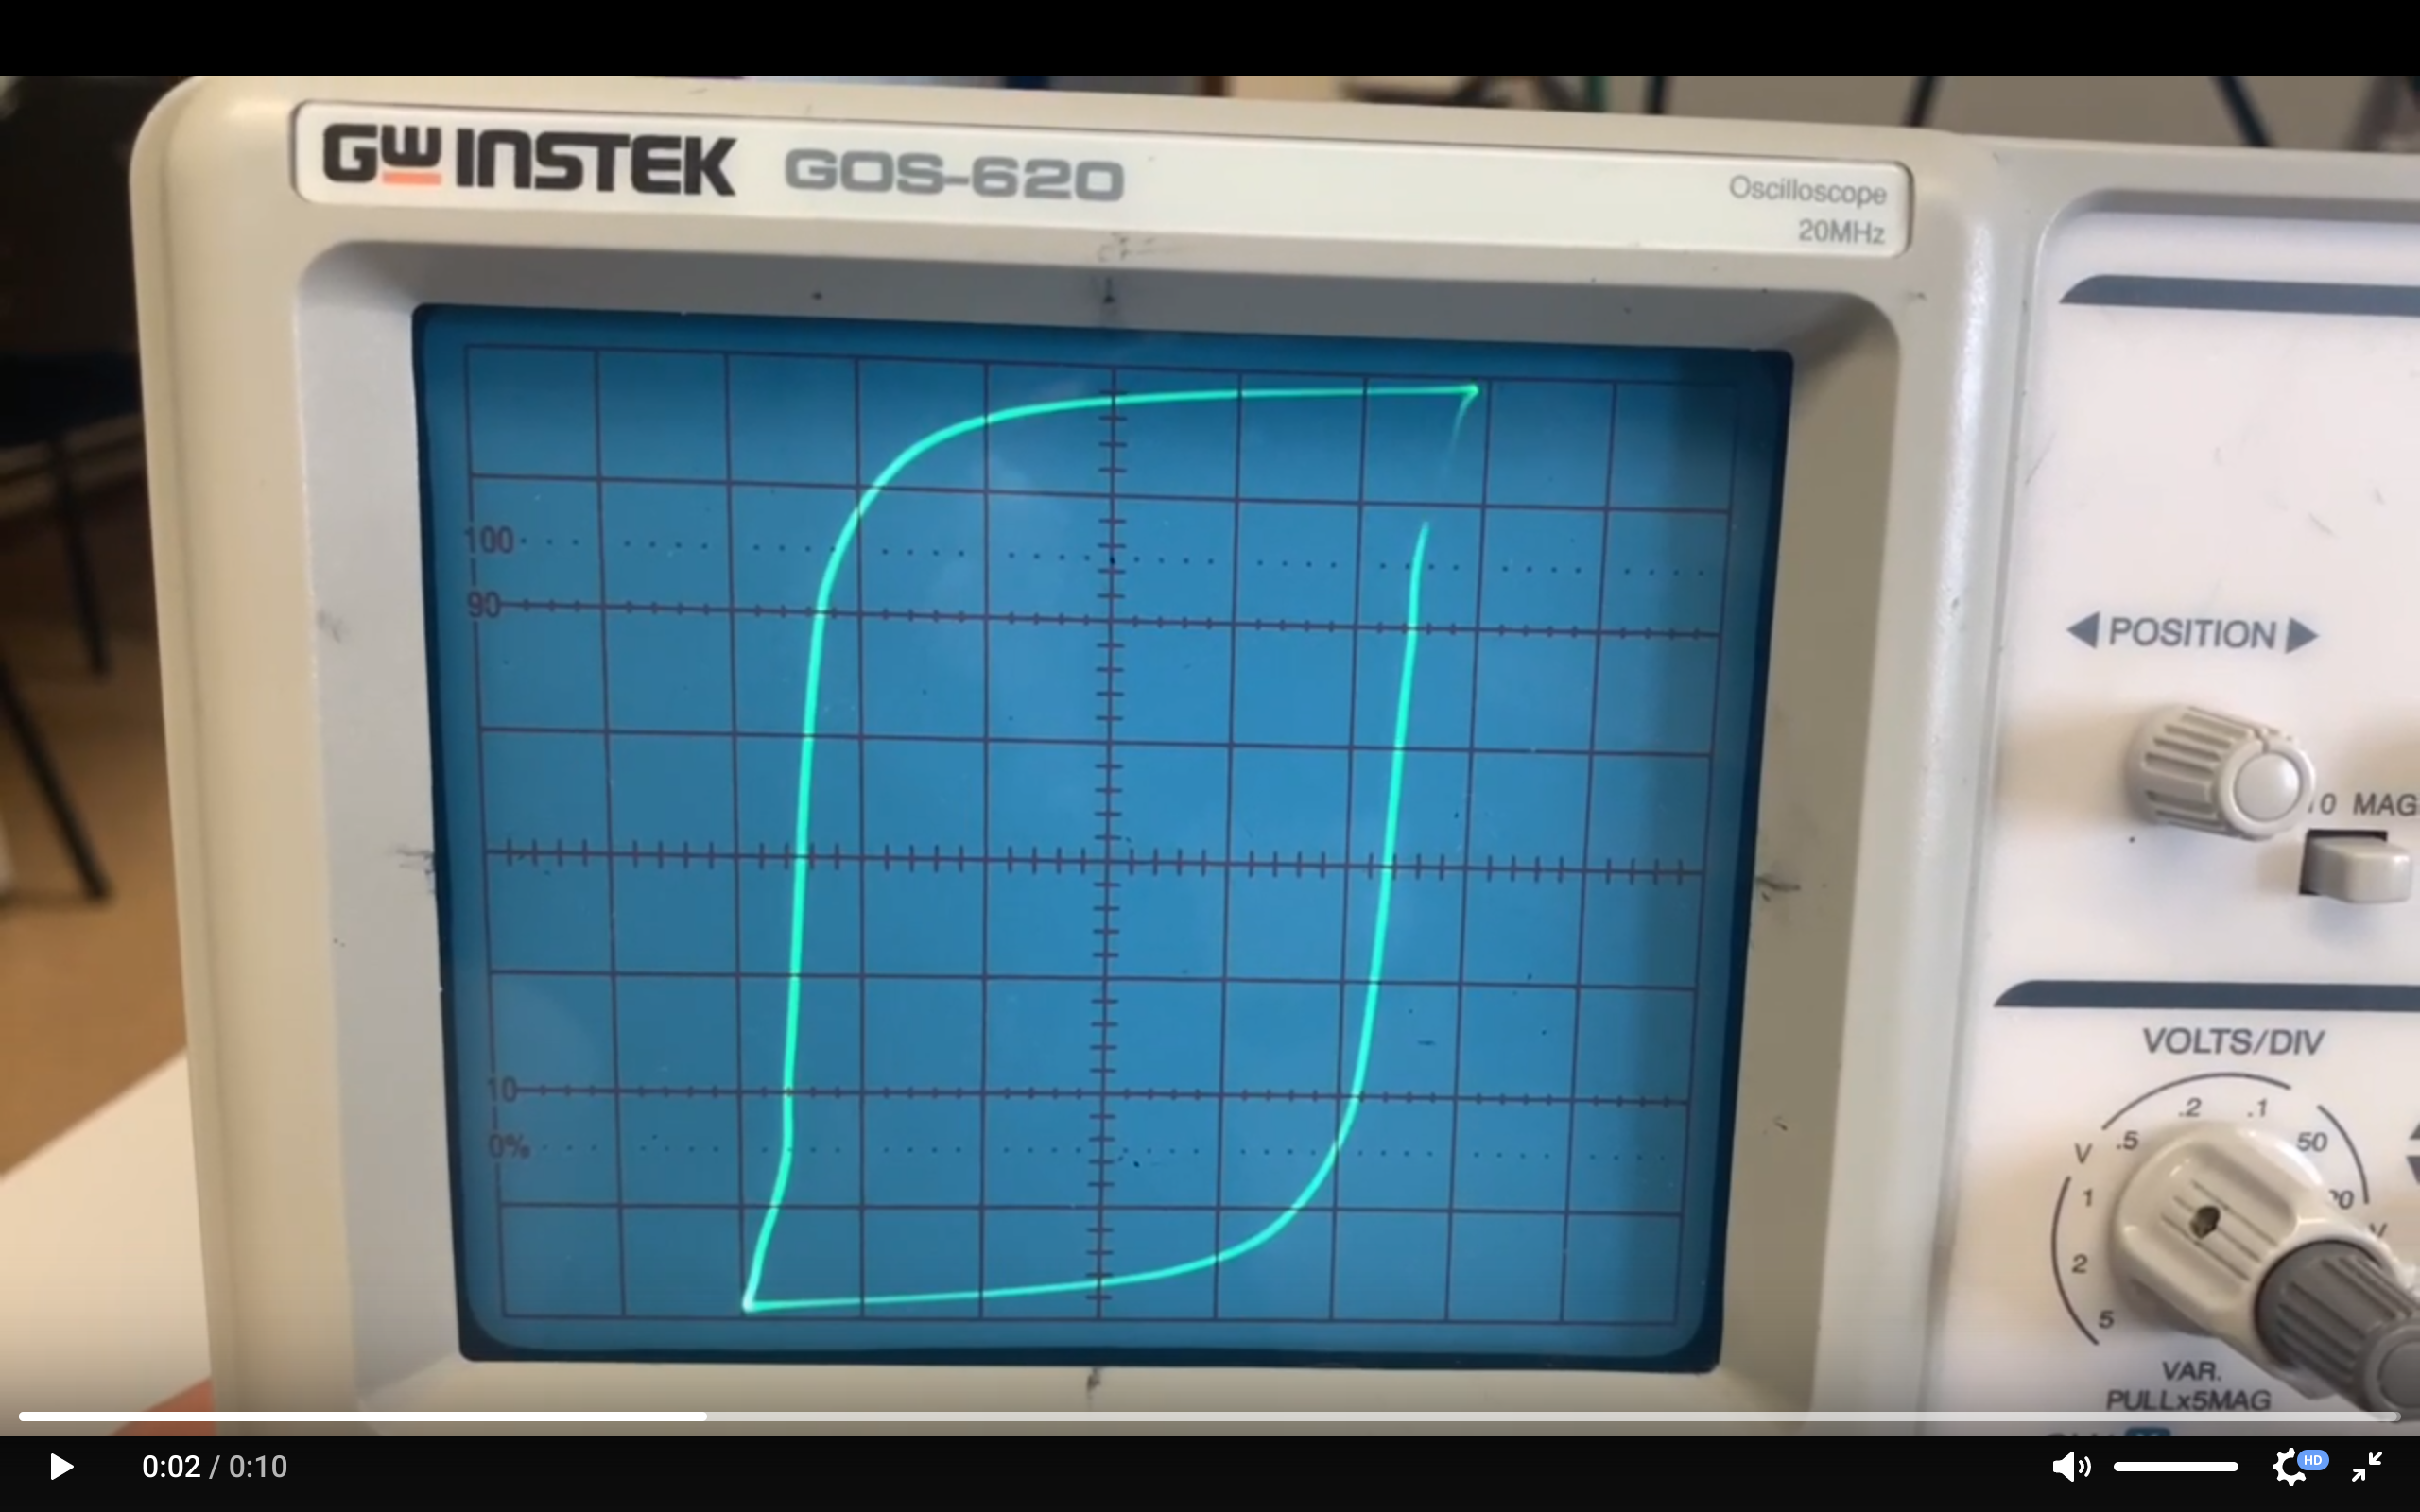
\includegraphics[width=0.55\textwidth]{permalloy_p.png}
    
    \textbf{Рис 2.2} Петля гистерезиса для пермаллоя
\end{center}

\begin{center}
    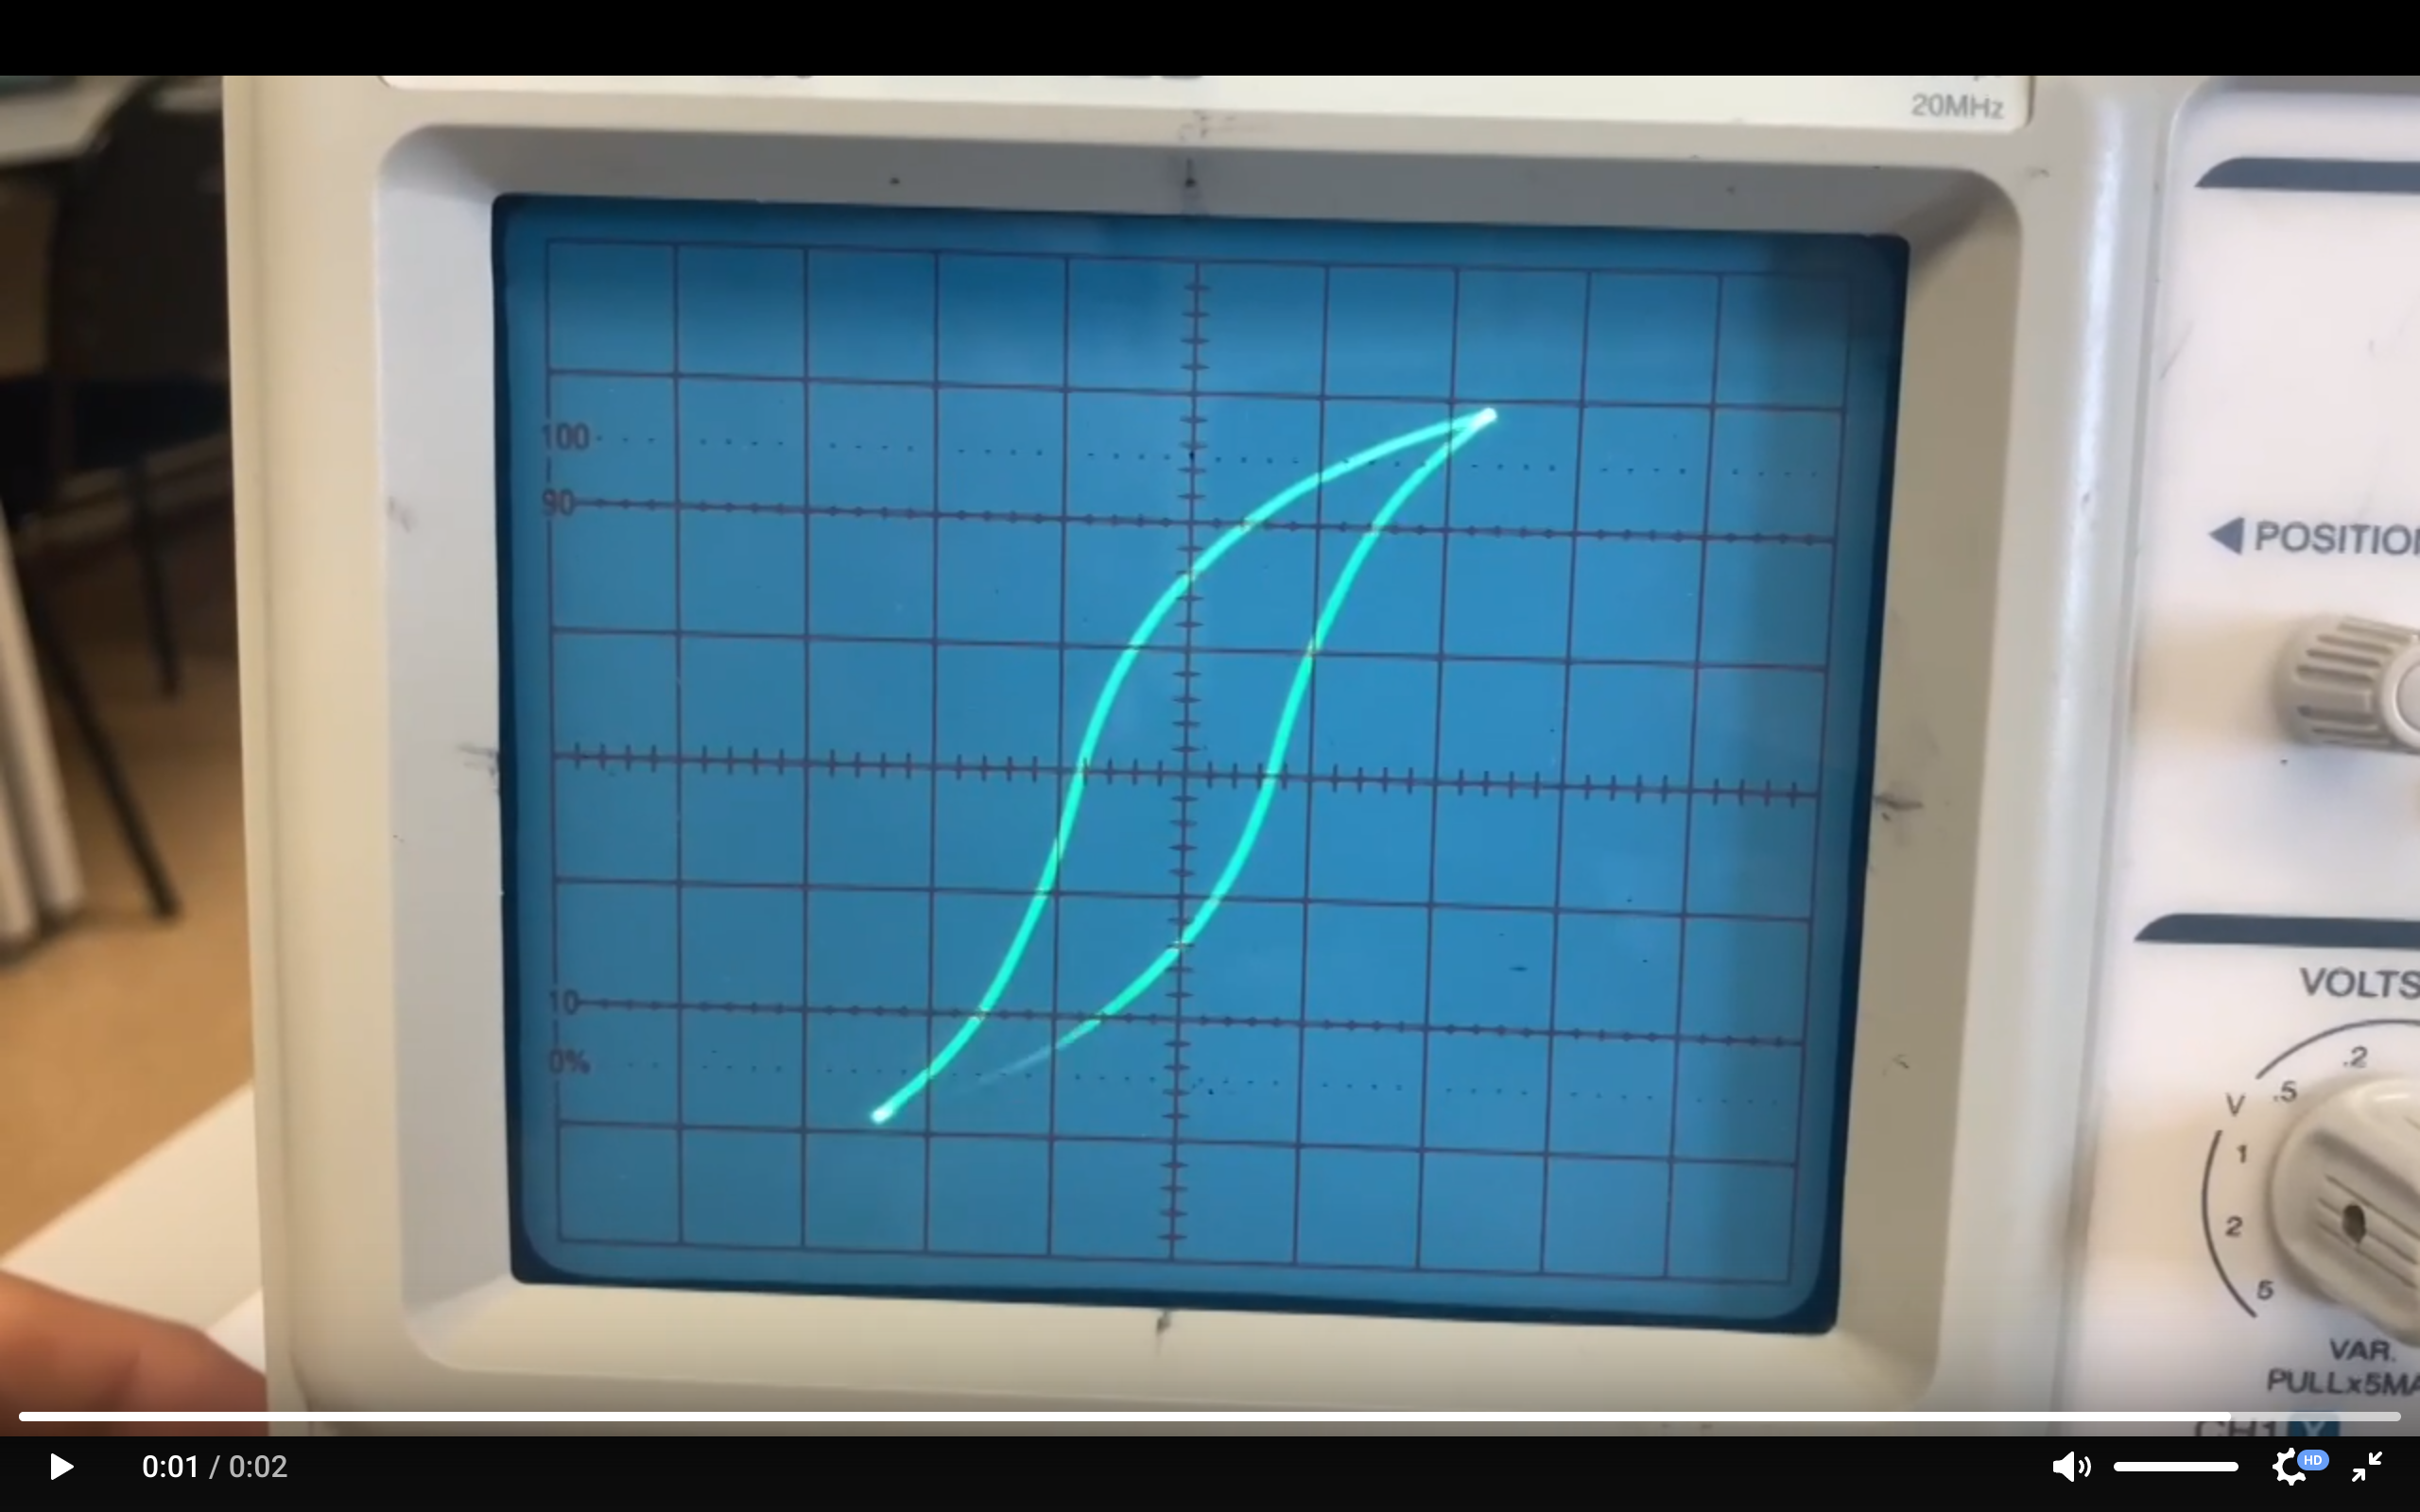
\includegraphics[width=0.55\textwidth]{k_ferrum_p.png}
    
    \textbf{Рис 2.3} Петля гистерезиса для кремниевого железа
\end{center}


\end{document}
